\documentclass{article}

\usepackage[scale=.8]{geometry}

\usepackage{tikz}
\usetikzlibrary{calc}

\pagestyle{empty}
\thispagestyle{empty}

\tikzset{
  regular polygon/.pic={
    \foreach \k in {1,...,#1}
    {
      \path[pic actions] ({(\k-1)*360/#1}:3) --  (\k*360/#1:3) -- ++({(\k-.5)*360/#1+90}:1);
      \path[pic actions] (\k*360/#1:3) ++({(\k-.5)*360/#1+90}:.6) arc[start angle={(\k-.5)*360/#1+90}, delta angle=360/#1, radius=.6];
      \path[pic actions] (\k*360/#1:3) ++({(\k+.5)*360/#1+90}:.4) arc[start angle={(\k+.5)*360/#1+90}, delta angle={180-360/#1}, radius=.4];
    }
  }
}

\begin{document}

\begin{tikzpicture}[remember picture, overlay]
\foreach[evaluate=\k as \vk using {(2*\k-1)/6}] \k in {1,2,3}
{
  \coordinate (l\k) at ($(current page.north west)!\vk!(current page.south west)$); 
  \coordinate (r\k) at ($(current page.north east)!\vk!(current page.south east)$); 
}
\foreach[
  evaluate=\k as \sides using \k+2,
  evaluate=\k as \yvalue using int((\k+1)/2),
  evaluate=\k as \xvalue using {1-(2*mod(\k,2)+1)/4}
] \k in {1,...,6}
{
  \pic[draw] at ($(l\yvalue)!\xvalue!(r\yvalue)$)  {regular polygon=\sides};
}
\end{tikzpicture}

\newpage

\begin{tikzpicture}[remember picture, overlay]
\foreach[evaluate=\k as \vk using {(2*\k-1)/6}] \k in {1,2,3}
{
  \coordinate (l\k) at ($(current page.north west)!\vk!(current page.south west)$); 
  \coordinate (r\k) at ($(current page.north east)!\vk!(current page.south east)$); 
}
\foreach[
  evaluate=\k as \sides using \k+8,
  evaluate=\k as \yvalue using int((\k+1)/2),
  evaluate=\k as \xvalue using {1-(2*mod(\k,2)+1)/4}
] \k in {1,...,6}
{
  \pic[draw] at ($(l\yvalue)!\xvalue!(r\yvalue)$)  {regular polygon=\sides};
}
\end{tikzpicture}

\end{document}
